\section{Der IEEE 802.15.4 Funkstandard}
IEEE 802.15.4 oder kurz 15.4 beschreibt einen Funkstandard, der bei geringer Datenrate die Leistungsaufnahme einzelner Teilnehmer möglichst weit zu reduzieren versucht. Das ist nötig, um den Anforderungen von Sensornetzwerken gerecht zu werden. \\
Durch den Standard werden der \ac{phy}- und \ac{mac}-Layer eines \ac{wpan} definiert. \\

\subsection{Teilnehmer und Topologien}
Dieses Kapitel deckt eigentlich Themen des Data Link Layers ab und ist im Kontext des entsprechenden Kapitels zu verstehen. Jedoch sind die Teilnehmer und Topologien des Netzwerks von so grundlegender Bedeutung, dass sie an dieser Stelle vorgezogen wurden. Alle Teilnehmer eines 15.4 \ac{pan} werden in zwei Kategorien eingeteilt:
\begin{itemize}
	\item Ein \ac{ffd} ist ein Teilnehmer mit vollständiger Implementierung von 15.4. Er kann alle Rollen annehmen.
	\item Ein \ac{rfd} hat reduzierte Fähigkeiten. Es kann nur mit einem FFD kommunizieren und somit nicht als Coordinator (siehe unten) auftreten.
\end{itemize}
15.4 ist gemäß IEEE für zwei verschiedene Netzwerk-Topologien ausgelegt:
\begin{itemize}
	\item Sterntopology
	\item Peer-to-Peer-Topology
\end{itemize}
\begin{figure}
	\centering
	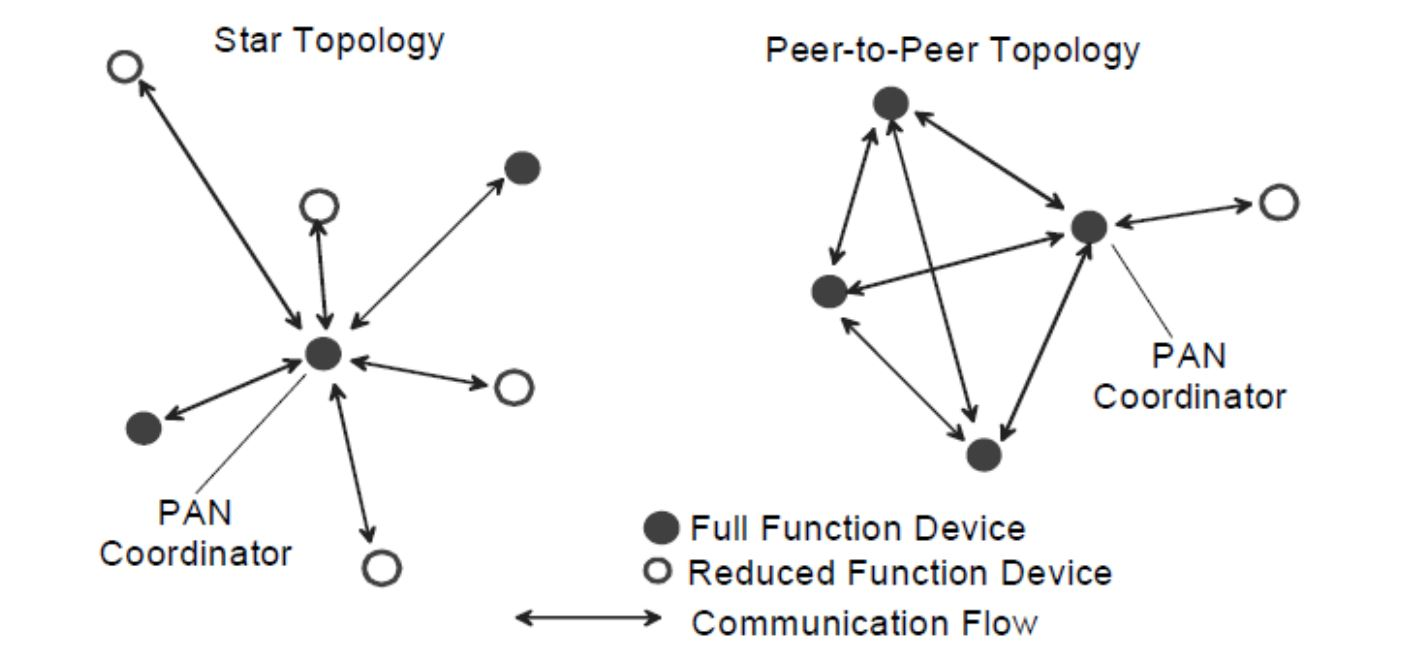
\includegraphics[width=0.7\textwidth]{Grafiken-Alex/topology.jpg}
	\caption{Topologien von 15.4-Netzwerken nach \cite[S.46]{ieee154}}
	\label{topology}
\end{figure}
In beiden Topologien existiert ein sogenannte \ac{pan}-Coordinator, der jedoch verschiedene Aufgaben übernimmt.\\
In einer Stern-Topologie ist der PAN-Coordinator der zentrale Kommunikationspunkt des Netzwerks. Alle Geräte kommunizieren nur mit ihm, was bedeutet, dass der Coordinator einen vergleichsweise hohen Energiebedarf hat. Die Teilnehmer hingegen müssen nur für ihre eigene Kommunikation aufwachen und können die restliche Zeit im Sleeping-Modus verbringen. Diese Topologie bietet sich an, wenn man einen netzbetriebenen Coordinator und mehrere batteriebetriebene Teilnehmer hat wie es z.B. in der Gebäudeautomatisierung oder bei \ac{pc} Peripheriegeräten der Fall ist.\\
Eine Peer-to-Peer-Topologie bietet sich offensichtlich für effizientes Routing an. Hierbei kommunizieren alle \ac{ffd} miteinander und \ac{rfd} als sogenannte Leafs mit einem \ac{ffd}. Anders als bei der Stern-Topologie ist somit der Coordinator nicht zentrale Kommunikationsstelle, sondern bietet Synchronisierungsservices o.ä. Diese Topologie bietet sich durch die Möglichkeit, Nachrichten per Multi-Hop zu routen im Bereich der Sensor-Netzwerke besonders an.\\
\begin{figure}
	\centering
	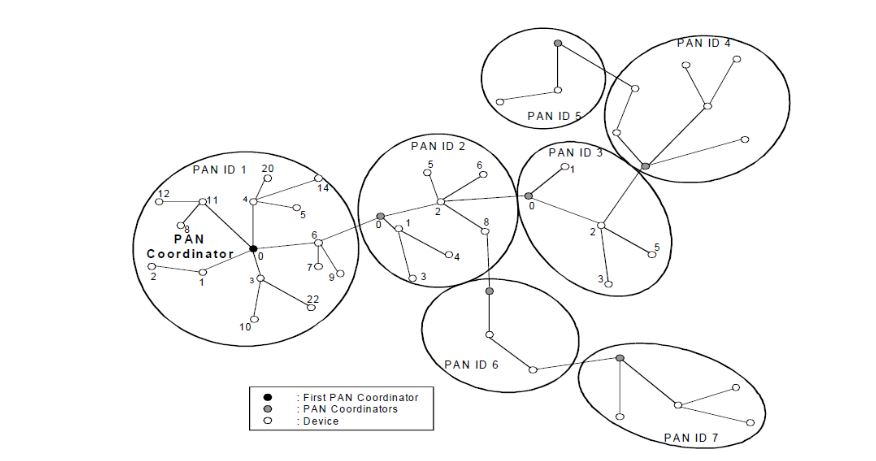
\includegraphics[width=\textwidth]{Grafiken-Alex/multicluster.jpg}
	\caption{Ein Multicluster Tree Netzwerk nach \cite[S.48]{ieee154}. Die Verbindungen zeigen nicht den Kommunikationsfluss, sondern Parent-Child-Beziehungen}
	\label{multicluster}
\end{figure}
Eine besondere Form der Peer-to-Peer-Technologie ist der Cluster Tree. Ein FFD beginnt einen neuen Cluster Tree, indem es eine freie PAN ID für das Netzwerk sucht und beginnt, sogenannte Beacons auszusenden. Das Device wird damit automatisch der Coordinator dieses Netzwerks. Ein Nachbar, der das Beacon empfängt, kann nun anfragen, am Netzwerk teilzunehmen. Erlaubt der Coordinator das, merkt er sich den Nachbarn als Child und dieser wiederum merkt sich den Coordinator als Parent. Der Nachbar beginnt nun seinerseits Beacons auszusenden, die weitere Geräte (auch solche, die nicht in direkter Reichweite des Coordinators sind) nutzen können, um dem Netzwerk teilzunehmen. Dadurch können große Netzwerke mit komplexen Routing-Tabellen entstehen. Darüber hinaus kann der PAN Coordinator einen Teilnehmer seines Netzwerks anweisen, ein eigenes Cluster zu konstruieren, bei dem er als PAN Coordinator auftritt. Dieser wiederum hält weiterhin Kontakt zu einem der Devices des originalen Netzwerks, wodurch große Multicluster-Netzwerke entstehen können. Grafik \ref{multicluster} zeigt ein solches Netzwerk. Durch diese Technik wird ein großer Netzwerkradius erreicht, wobei die Latenz einer Nachricht mit der Größe des Netzwerks zunimmt.\\

\subsection{Physical Layer}
\subsubsection{Genutzte Frequenzbänder}
15.4 nutzt die folgenden Frequenzbänder:
\begin{itemize}
	\item 2,4-2,4835 GHz ISM Band (16 Kanäle) weltweit
	\item 902-928 MHz ISM Band (10 Kanäle) in den USA
	\item 868-868,6 MHz Band (1 Kanal) in Europa
\end{itemize}
Dabei wird im 902MHz-Band ein Kanalabstand von 2 MHz und im 2,4GHz-Band ein Kanalabstand von 5 MHz eingesetzt. Die Kanäle werden mit Channel 0 (868 MHz), Channel 1-10 (902 MHz) und Channel 11-26 (2,4 GHz) bezeichnet.
\subsubsection{Genutzte Spreiz- und Modulationsverfahren}
Zum Verständnis der Modulation des Physical Layer durch 15.4 sind Kenntnisse über verschiedene Modulationsverfahren nötig. Diese sind im Folgenden kurz beschrieben. \\

\textbf{\ac{dsss}} \\
\begin{figure}
	\centering
	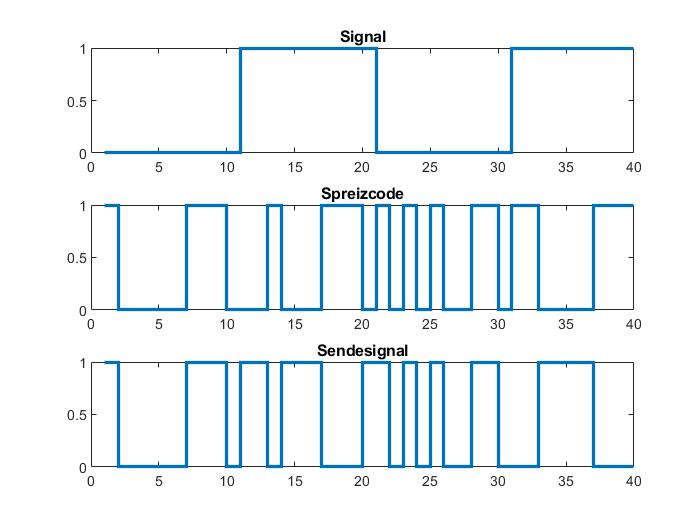
\includegraphics[width=0.7\textwidth]{Grafiken-Alex/dsss.jpg}
	\caption{Ein per DSSS gespreiztes Signal}
	\label{dsss}
\end{figure}
Das \acf{dsss} - ein sogenanntes Spreizverfahren - dient dazu, den Bitstrom auf ein breiteres Frequenzband zu spreizen. Dabei wird die ursprüngliche Bitfolge auf einen pseudo-zufällige Subbit-Strom moduliert. Die einzelnen Subbits dieses Stroms werden Chips genannt, der Strom Chipfolge oder Spreizcode.\\
In Abbildung \ref{dsss} wird das Signal mit einem Spreizcode unter Verwendung der XOR-Funktion gespreizt. Auf jedes Bit des Signals kommen dabei 10 Chips, wodurch eine Chiprate erreicht wird, die zehn Mal so hoch wie die Bitrate ist. Dieses Verhältnis wird auch Spreizfaktor genannt.\\
Sinn der DSSS ist es, ein Signal unempfindlicher schmalbandiger Störungen zu machen. Offensichtlich muss dem Empfänger zu Demodulation entweder der Spreizcode oder - da er pseudo-zufällig ist - der Generator zur Erstellung des Spreizcodes bekannt sein.\\

\textbf{\ac{bpsk}} \\
\begin{figure}
	\centering
	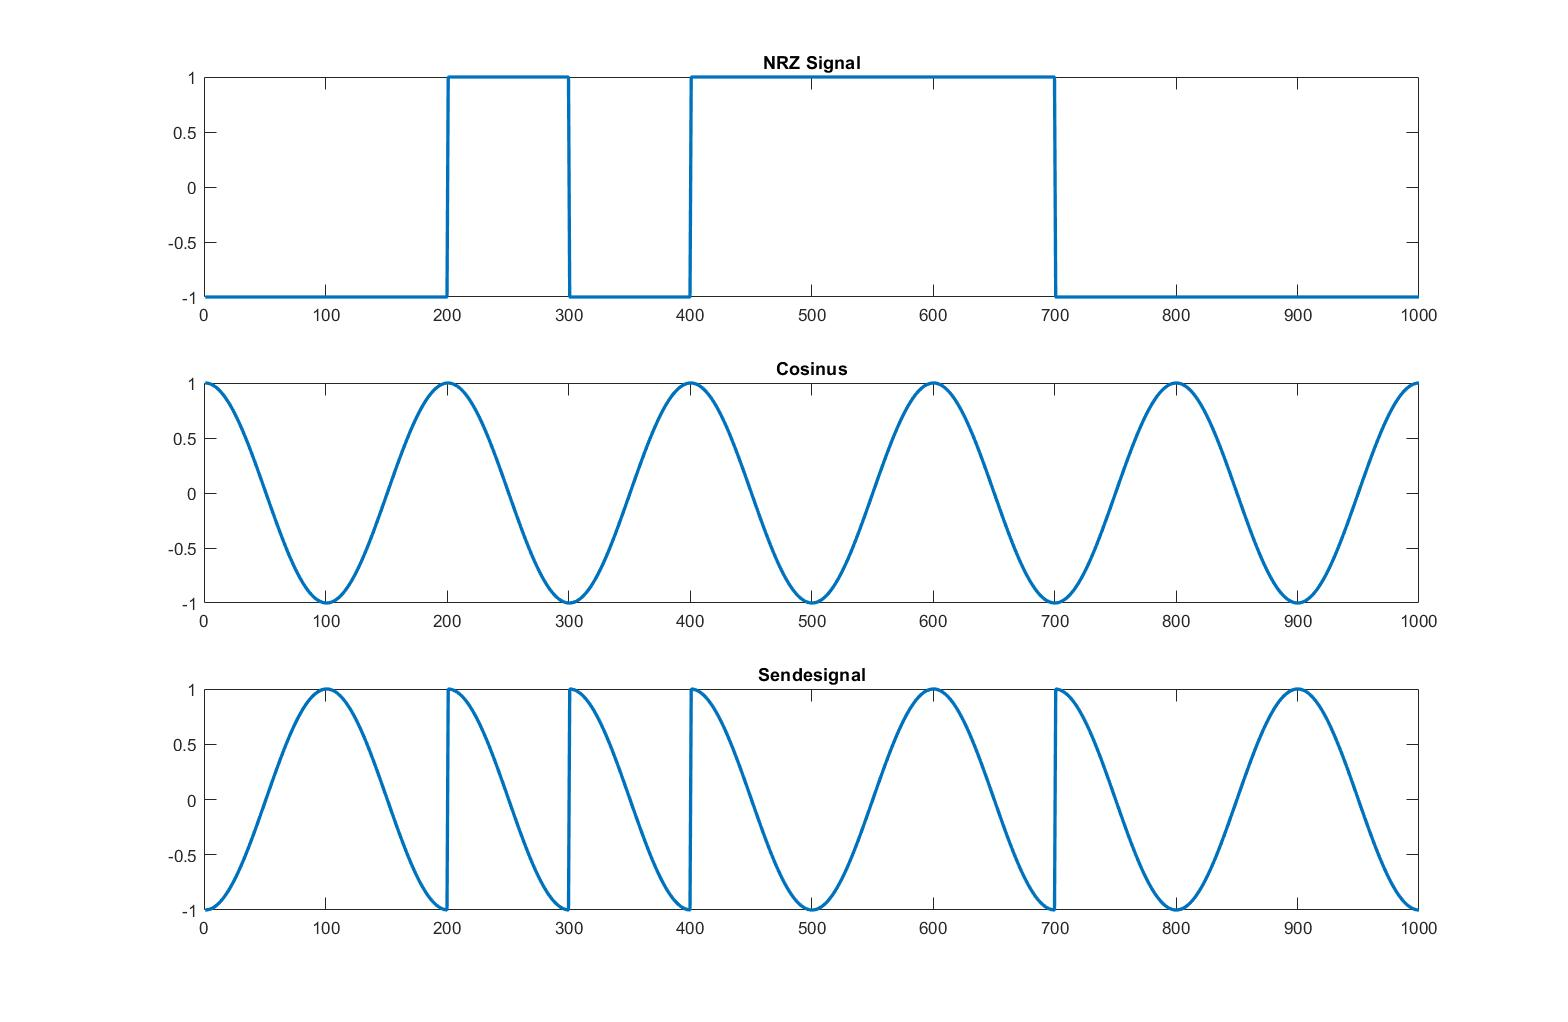
\includegraphics[width=0.7\textwidth]{Grafiken-Alex/bpsk.jpg}
	\caption{Ein BPSK-moduliertes Signal mit einer Cosinus-Schwingung als Träger}
	\label{bpsk}
\end{figure}
Die \acf{bpsk} ist die einfachste Form des Phase-Shift-Keyings. Die Bitfolge wird dabei als bipolares \ac{nrz} dargestellt und daraufhin mit dem Trägersignal multipliziert. Grafik \ref{bpsk} zeigt das Prinzip. \\

\textbf{\ac{oqpsk}}\\
\begin{figure}
	\centering
	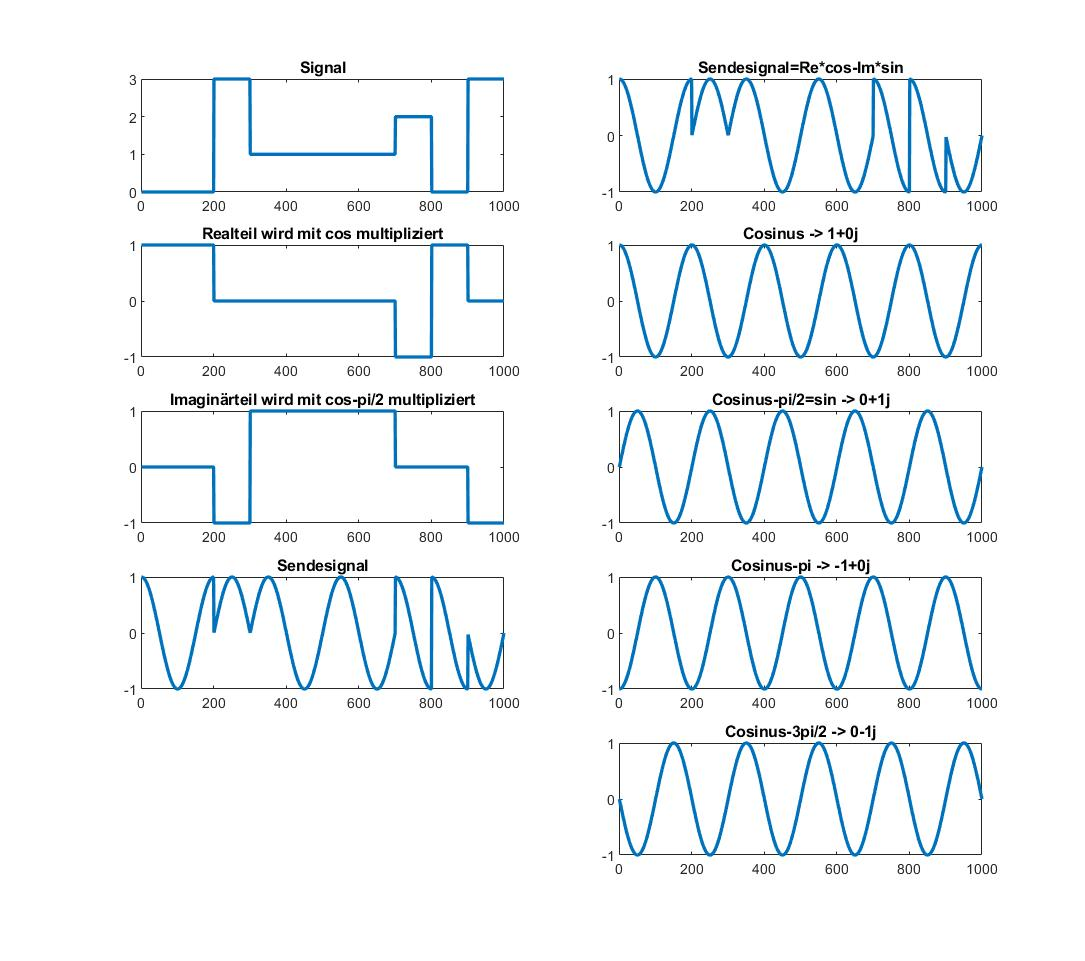
\includegraphics[width=\textwidth]{Grafiken-Alex/qpsk.jpg}
	\caption{Beispielhafte Erzeugung eines Sendesignals mit QPSK (links) und das Sendesignal im Vergleich mit phasenverschobenen Cosinus-Schwingungen (rechts).}
	\label{qpsk}
\end{figure}
Das \acf{oqpsk} ist eine komplexere Form des Phase-Shift-Keyings, bei der mit jedem Symbol ein Informationsgehalt von zwei Bits übertragen wird. Zunächst wird normales QPSK betrachtet. Hierbei wird der Bitstrom aufgeteilt in einen Real- und einen Imaginärbitstrom, wobei jedes zweite Bit in den Imaginärbitstrom fließt. Diese Ströme gehen daraufhin als Eingänge in einen \ac{qam} Modulator, welcher sie mit einem Cosinus (Real) bzw. Sinus (Imaginär) multipliziert und die Resultate subtrahiert, um das Sendesignal zu bilden.\\
Eine sinnvollere Aufteilung wird dadurch erreicht, dass der Bitstrom in der komplexen Zahlenebene so gemappt wird, dass der komplexe Zahlenstrom, der durch das Mapping entsteht gleichmäßig um den Ursprung verteilt ist. Das kann beispielsweise dadurch realisiert werden, dass die Zahlenfolge 00 als 0+0j dargestellt wird, die Zahlenfolge 01 als 0+1j usw. Häufig werden auch die resultierenden Werte um $\pi/4$ verschoben, also 00 auch 1+1j gemappt, 01 auf -1+1j usw.\\
Statt eines binären Zahlenstroms wird häufig ein Zahlenstrom mit Werten im Bereich [0,3] eingesetzt. Dieser hat die halbe Symbolrate des binären Stroms, aber statt einem zwei Bit/Symbol, wodurch wiederum die gleiche Bitrate erreicht wird. Der Vorteil besteht darin, dass er die gleiche Symbolrate wie der resultierende komplexe Zahlenstrom hat.\\
Die Erzeugung eines Signals mit QPSK ist in Grafik \ref{qpsk} anschaulich dargestellt.\\
Im Sendesignal ist klar erkennbar, dass bei Nulldurchgängen, also zum Beispiel von 1+0j zu -1+0j große Phasensprünge resultieren. Weil man dies vermeiden will, verschiebt man Real- und Imaginärteil des komplexen Signals um $\pi/2$ und bezeichnet das Resultat als Offset-QPSK oder kurz O-QPSK.\\

\subsubsection{Konkretes Modulationsverfahren}
\begin{figure}
	\centering
	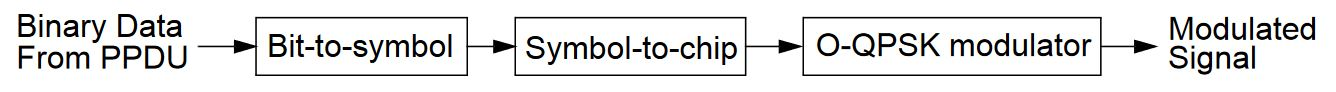
\includegraphics[width=\textwidth]{Grafiken-Alex/modulation.jpg}
	\caption{Ablauf der Modulation bei 15.4 aus \cite[S.412]{ieee154}}
	\label{modulation}
\end{figure}
Tatsächlich benutzt 15.4 eine Kombination aus DSSS und O-QPSK im 2,4GHz-Band und DSSS kombiniert mit BPSK in den restlichen Bändern. Der Ablauf der Modulationsverfahren ist in Abbildung \ref{modulation} dargestellt. Zunächst wird der Datenstrom in Oktette aufgeteilt. Jedes Oktett wird wiederum in zwei Symbole aufgeteilt, wobei die LSB (b0,b1,b2,b3) ein Symbol bilden und die MSB (b4,b5,b6,b7) ein anderes. Es ist darauf zu achten, dass das Symbol der LSB zuerst versendet wird.\\
Weil ein Symbol aus 4 bit besteht, kann es 16 verschiedene Werte annehmen. Entsprechend des Werts des Symbols wird einer von 16 verschiedenen, zueinander orthogonalen Spreizcodes verwendet, die im 2,4GHz-Band eine Länge von 32 Chips und in den restlichen Bändern eine Länge von 16 Chips haben und in der IEEE-Norm für das 2,4GHz-Band wie folgt festgelegt sind.\cite[S.413]{ieee154}\\
\begin{center}
	\begin{tabular}{cc}
		\textbf{Wert des Symbols} & \textbf{32-bit Spreizcode} \\
		0 &1 1 0 1 1 0 0 1 1 1 0 0 0 0 1 1 0 1 0 1 0 0 1 0 0 0 1 0 1 1 1 0\\
		1&1 1 1 0 1 1 0 1 1 0 0 1 1 1 0 0 0 0 1 1 0 1 0 1 0 0 1 0 0 0 1 0\\
		2&0 0 1 0 1 1 1 0 1 1 0 1 1 0 0 1 1 1 0 0 0 0 1 1 0 1 0 1 0 0 1 0\\
		3&0 0 1 0 0 0 1 0 1 1 1 0 1 1 0 1 1 0 0 1 1 1 0 0 0 0 1 1 0 1 0 1\\
		4&0 1 0 1 0 0 1 0 0 0 1 0 1 1 1 0 1 1 0 1 1 0 0 1 1 1 0 0 0 0 1 1\\
		5&0 0 1 1 0 1 0 1 0 0 1 0 0 0 1 0 1 1 1 0 1 1 0 1 1 0 0 1 1 1 0 0\\
		6&1 1 0 0 0 0 1 1 0 1 0 1 0 0 1 0 0 0 1 0 1 1 1 0 1 1 0 1 1 0 0 1\\
		7&1 0 0 1 1 1 0 0 0 0 1 1 0 1 0 1 0 0 1 0 0 0 1 0 1 1 1 0 1 1 0 1\\
		8&1 0 0 0 1 1 0 0 1 0 0 1 0 1 1 0 0 0 0 0 0 1 1 1 0 1 1 1 1 0 1 1\\
		9&1 0 1 1 1 0 0 0 1 1 0 0 1 0 0 1 0 1 1 0 0 0 0 0 0 1 1 1 0 1 1 1\\
		10&0 1 1 1 1 0 1 1 1 0 0 0 1 1 0 0 1 0 0 1 0 1 1 0 0 0 0 0 0 1 1 1\\11&0 1 1 1 0 1 1 1 1 0 1 1 1 0 0 0 1 1 0 0 1 0 0 1 0 1 1 0 0 0 0 0\\
		12&0 0 0 0 0 1 1 1 0 1 1 1 1 0 1 1 1 0 0 0 1 1 0 0 1 0 0 1 0 1 1 0\\
		13&0 1 1 0 0 0 0 0 0 1 1 1 0 1 1 1 1 0 1 1 1 0 0 0 1 1 0 0 1 0 0 1\\
		14&1 0 0 1 0 1 1 0 0 0 0 0 0 1 1 1 0 1 1 1 1 0 1 1 1 0 0 0 1 1 0 0\\
		15&1 1 0 0 1 0 0 1 0 1 1 0 0 0 0 0 0 1 1 1 0 1 1 1 1 0 1 1 1 0 0 0\\
	\end{tabular}
\end{center}

Für die restlichen Bänder werden die Symbole auf folgende Spreizcodes gemappt. \cite[S.414]{ieee154}
\begin{center}
	\begin{tabular}{cc}
		\textbf{Wert des Symbols} & \textbf{16-bit Spreizcode} \\
		0&0 0 1 1 1 1 1 0 0 0 1 0 0 1 0 1\\
		1&0 1 0 0 1 1 1 1 1 0 0 0 1 0 0 1\\
		2&0 1 0 1 0 0 1 1 1 1 1 0 0 0 1 0\\
		3&1 0 0 1 0 1 0 0 1 1 1 1 1 0 0 0\\
		4&0 0 1 0 0 1 0 1 0 0 1 1 1 1 1 0\\
		5&1 0 0 0 1 0 0 1 0 1 0 0 1 1 1 1\\
		6&1 1 1 0 0 0 1 0 0 1 0 1 0 0 1 1\\
		7&1 1 1 1 1 0 0 0 1 0 0 1 0 1 0 0\\
		8&0 1 1 0 1 0 1 1 0 1 1 1 0 0 0 0\\
		9&0 0 0 1 1 0 1 0 1 1 0 1 1 1 0 0\\
		10&0 0 0 0 0 1 1 0 1 0 1 1 0 1 1 1\\
		11&1 1 0 0 0 0 0 1 1 0 1 0 1 1 0 1\\
		12&0 1 1 1 0 0 0 0 0 1 1 0 1 0 1 1\\
		13&1 1 0 1 1 1 0 0 0 0 0 1 1 0 1 0\\
		14&1 0 1 1 0 1 1 1 0 0 0 0 0 1 1 0\\
		15&1 0 1 0 1 1 0 1 1 1 0 0 0 0 0 1\\
	\end{tabular}
\end{center}
\begin{figure}
	\centering
	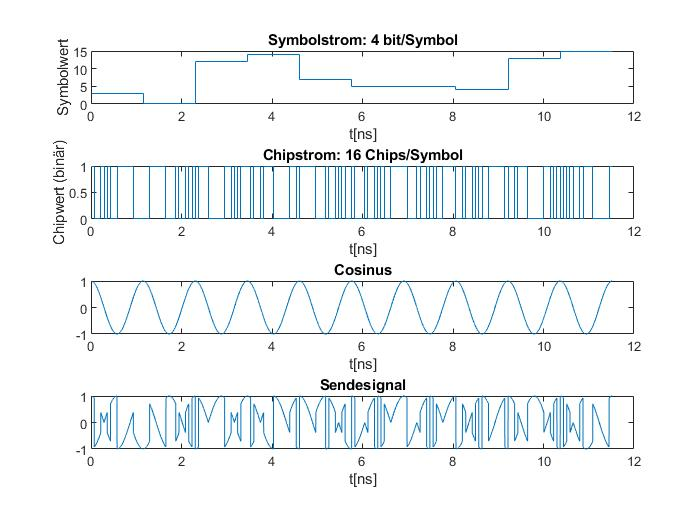
\includegraphics[width=\textwidth]{Grafiken-Alex/154modulation.jpg}
	\caption{Die vollständige Modulation eines Symbolstroms auf einen 868MHz-Träger unter Verwendung eines Alphabets mit 16 Chips/Symbol und BPSK als Modulationsart}
	\label{154modulation}
\end{figure}

Die so entstandenen Chipströme werden nun mit einem O-QPSK bzw. BPSK-Modulator moduliert. Zur Veranschaulichung zeigt Grafik \ref{154modulation} die gesamte Modulation eines Symbolstroms - dieser setzt sich aus 4 Bit/Symbol zusammen - zum analogen Sendesignal. \\

\subsection{Data Link Layer}
\begin{figure}
	\centering
	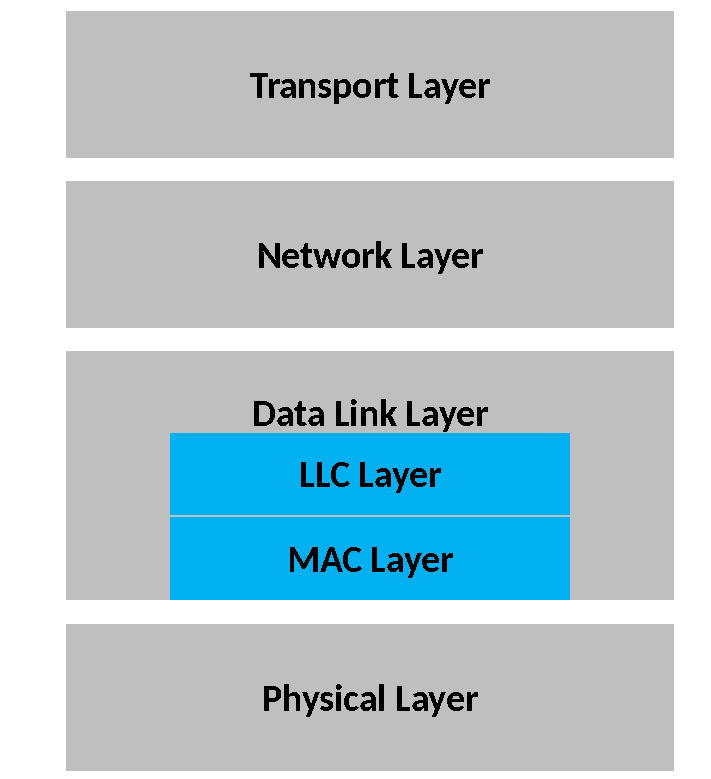
\includegraphics[width=0.5\textwidth]{Grafiken-Alex/ieee-osi.pdf}
	\caption{Die Unterteilung des Data Link Layers in LLC und MAC nach Norm des IEEE}
	\label{ieee-osi}
\end{figure}
Die IEEE unterteilt das aus dem OSI-Modell bekannte Data Link Layer in zwei Sublayer, die \ac{llc} Layer und \acf{mac} Layer heißen. Dabei ist der MAC-Layer in der Hirarchie unterhalb des LLC-Layers angesiedelt und wird häufig als Layer 2a, letzteres als Layer 2b bezeichnet. Grafik \ref{ieee-osi} zeigt die Aufteilung des Data Link Layers in LLC und MAC anschaulich.\\
Der LLC-Layer ist in IEEE 802.2 für alle Protokolle der 802-Norm definiert, hat sich aber in der Realität nicht durchgesetzt, weshalb der Network-Layer direkt auf den MAC-Layer zugreift. \cite{bartusch}IEEE 802.15.4 spezifiziert aus diesem Grund nur den MAC-Layer, weshalb im folgenden nicht auf die LLC-Schicht eingegangen wird. Die Begriffe Data Link Layer und Medium Access Layer können demnach im Kontext dieses Dokuments als Synonyme angesehen werden.
\subsubsection{MAC-Layer}
Wie bei vielen Funkübertragungstechniken üblich verwendet 15.4 den \ac{csmaca} Algorithmus. Ziel dabei ist es, Kollisionen auf dem Kanal zu vermeiden statt sie wie bei \ac{csmacd} zu erkennen und sich gegebenenfalls zurückzuziehen (z.B. per Arbitrierung). Die Nutzung von CSMA/CA bedeutet für einzelne Teilnehmer, dass sie zunächst auf dem Kanal lauschen müssen, um zu erkennen, ob dort gerade eine Kommunikation stattfindet und erst, wenn die Sendeleistung auf diesem Kanal einen bestimmten Wert unterschreitet - ergo es ist nur Rauschen vorhanden - senden darf. Abhängig vom genutzten Frequenzband kann er die verschiedenen zur Verfügung stehenden Kanäle analysieren und sich einen freien Kanal suchen (im 2,4-GHz-Band stehen immerhin 16 Kanäle zur Verfügung). \\

\textbf{MAC-Adresse}\\
Zur eindeutigen Identifizierung jedes Teilnehmers teilt sich jeder eine 8 Byte lange MAC-Adresse zu. Diese wird schon beim Flashen der Software festgelegt und bleibt somit über die Lebensdauer des Geräts bestehen. Die vollständige MAC-Adresse wird nach dem von der IEEE standardisierten Format \ac{eui64} erzeugt. Die ersten drei Bytes kennzeichnen demnach den Gerätehersteller, während die restlichen Bytes durch das Unternehmen selbst vergeben werden. Dadurch wird gewährleistet, dass jedes Gerät eine global einmalige MAC-Adresse erhält. \\
Weil eine 8 Byte lange MAC-Adresse offensichtlich gerade unter Berücksichtigung des gerade mal bis zu 127 Byte großen Frames eines 15.4 Pakets einen zu großen Overhead erzeugt - und die globale Einmaligkeit aufgrund der lokalen Beschränktheit eines Personal Area Networks ohnehin nicht relevant ist - kann der Teilnehmer sich bei der Anmeldung im Netzwerk durch den PAN Coordinator eine Kurzadresse (engl. Short Address) von zwei Bytes zuweisen lassen. Das beschränkt zwar die maximale Teilnehmerzahl eines Netzwerks auf 65535 Teilnehmer, jedoch sind Sensornetzwerke dieser Größenordnung ohnehin nicht realistisch. Im Jahr 2015 dürfte das größte Sensornetzwerk im Bereich von 1000 Sensorknoten gelegen haben. \cite{schiessleiot} \\

\textbf{Beacon und Non-Beacon Mode}\\
Im MAC-Layer gibt es zwei Möglichkeiten, den Kanalzugriff zu organisieren. Die einfachere davon ist der Non-Beacon Mode, bei dem die Teilnehmer durch simplen Einsatz des CSMA/CA Algorithmus wie oben beschrieben auf den Kanal zugreifen können. Das sorgt für eine sehr einfache Implementierung des MAC Layers, verzichtet aber auf die organisatorischen Vorteile des Beacon Modes.\\
Dieser setzt auf sogenannte Superframes. Ein Superframe ist ein Zeitrahmen, der mehrere Frames (=15.4 Pakete) überdauert. Ein Superframe wird durch das Aussenden eines Beacons durch den PAN Coordinator begonnen und endet mit dem Beginn des nächsten Superframes. Innerhalb eines Superframes lassen sich nun aktive Phasen und inaktive Phasen definieren, sodass den Teilnehmern des Netzwerks ermöglicht wird, zu gewissen Zeitpunkten in den Sleep-Modus zu gehen. Deshalb wird die inaktive Phase auch als Sleep Period bezeichnet.\\
\begin{figure}
	\centering
	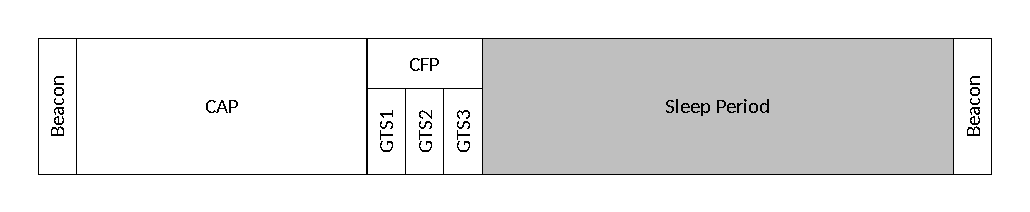
\includegraphics[width=\textwidth]{Grafiken-Alex/superframe.pdf}
	\caption{Inhalte eines Superframes bei Nutzung von 15.4 im Beacon Mode}
	\label{superframe}
\end{figure}
Die aktive Phase lässt sich weiter in \ac{cap} und \ac{cfp} unterteilen. \cite{superframestructure}. In ersterer ist der Kanal für alle Teilnehmer verfügbar und darf unter Verwendung des CSMA/CA-Algorithmus genutzt werden. Ein Teilnehmer - im Übrigen auch Node genannt - kann den Channel durch zweimaliges Durchführen der \ac{caa} Methode - hierbei lauscht er auf dem Kanal, ob Kommunikation stattfindet - erforschen und darf daraufhin - vorausgesetzt es findet aktuell keine Kommunikation statt - seine Daten senden. \cite{sarodeslottedscmaca} Es ist darauf zu achten, dass es sich hierbei um ein Slotted CSMA/CA handelt und deshalb CAA zu Beginn eines Slots durchgeführt werden muss. \\
Die CFP Periode wird in \ac{gts} unterteilt. Einem Teilnehmer kann also ein Slot zugewiesen werden, während dem er den garantierten alleinigen Zugriff auf den Kanal hat. Dabei ist anzunehmen, dass Nodes geringer Priorität ihre Daten während der CAP versenden und Nodes hoher Priorität eine GTS in der CFP zugewiesen bekommen. Nach Abschluss der CFP beginnt die Sleep Period. Die Länge der jeweiligen Perioden und ihre Existenz - CFP und Sleep Period sind optional - teilt der PAN Coordinator mit dem Inhalt des Beacons mit. Die ganze Struktur eines Superframes ist in Abbildung \ref{superframe} dargestellt. Es ist im Übrigen darauf zu achten, dass die CFP maximal sieben GTS bereitstellen darf. Das resultiert darauf, dass ein Superframe eine maximale Länge von 16 Slots hat, wobei 9 Slots für CAP bereitgestellt werden müssen.

\subsection{Datenrahmen}
Die Datenrahmen können eigentlich den einzelnen Schichten zugeordnet werden, sind aber so miteinander verbunden, dass es zum Verständnis beiträgt, sie in einem Kapitel zu besprechen. Aus diesem Grund werden sie in diesem Kapitel aufgeteilt nach der jeweiligen Schicht behandelt. Es ist weiterhin darauf zu achten, dass der ganze Rahmen einer jeweiligen Schicht als \ac{pdu} bezeichnet wird und die jeweilige Payload als \ac{sdu}.

\subsubsection{\ac{ppdu}}
\begin{figure}
	\centering
	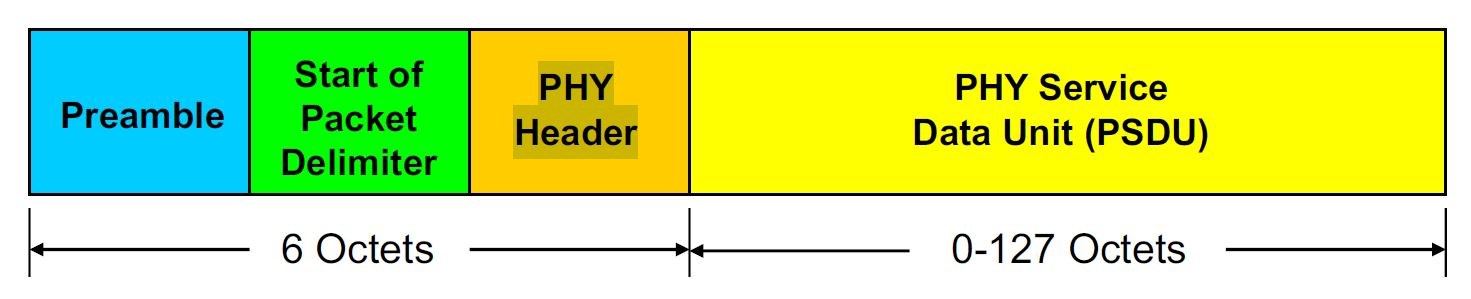
\includegraphics[width=\textwidth]{Grafiken-Alex/ppdu.jpg}
	\caption{Der Frame des Physical Layers in 15.4 aus \cite{rubinstein}}
	\label{ppdu}
\end{figure}
Ein Paket besteht zunächst aus dem Frame des Physical Layers. Dieser enthält eine 8 Byte lange Präambel, die zur Synchronisation dient, einen 1 Byte langen Start of Frame und den 1 Byte langen PHY Header, der die Länge des \ac{psdu} beschreibt. Daraufhin folgen die Nutzdaten, die eine Länge von bis zu 127 Byte haben können. Die ganze PPDU ist in Grafik \ref{ppdu} zu sehen. 
\subsubsection{\ac{mpdu}}
\begin{figure}
	\centering
	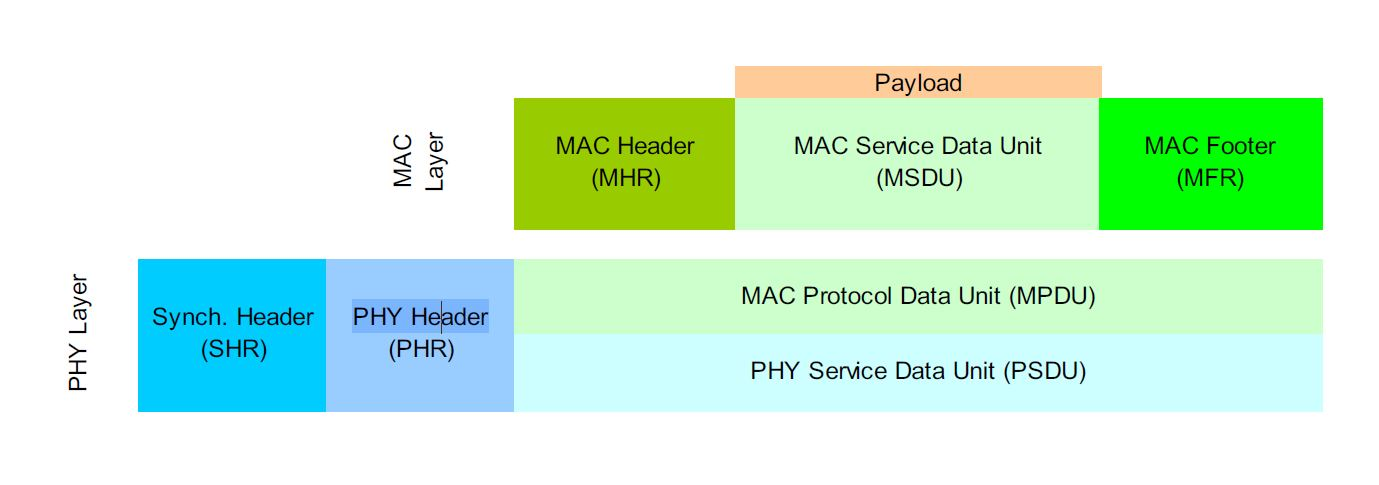
\includegraphics[width=\textwidth]{Grafiken-Alex/mpdu.jpg}
	\caption{Der Frame des MAC Layers (oben) und seine Einordnung in den Frame des PHY Layers (unten) in 15.4 aus \cite{rubinstein}}
	\label{mpdu}
\end{figure}
Da die MAC Schicht direkt über dem PHY Layer liegt, stellt die \acf{mpdu} gleichzeitig die Payload des Phy Frames und somit die \acf{psdu} dar. Abbildung \ref{mpdu} zeigt dieses Prinzip. \\
Die MPDU als solches besteht aus einem MAC Header, der \acf{msdu} und einem MAC Footer. Die MSDU ist die Payload des MAC Layers und kann Frames höherer Schichten enthalten.


